\section{Problem 4}
\subsection{Source routing algorithm}

To simplify the notations when describing paths, labels are assigned to paths as shown in Figure \ref{fig:graph}.

\begin{figure}[h]
    \centering
    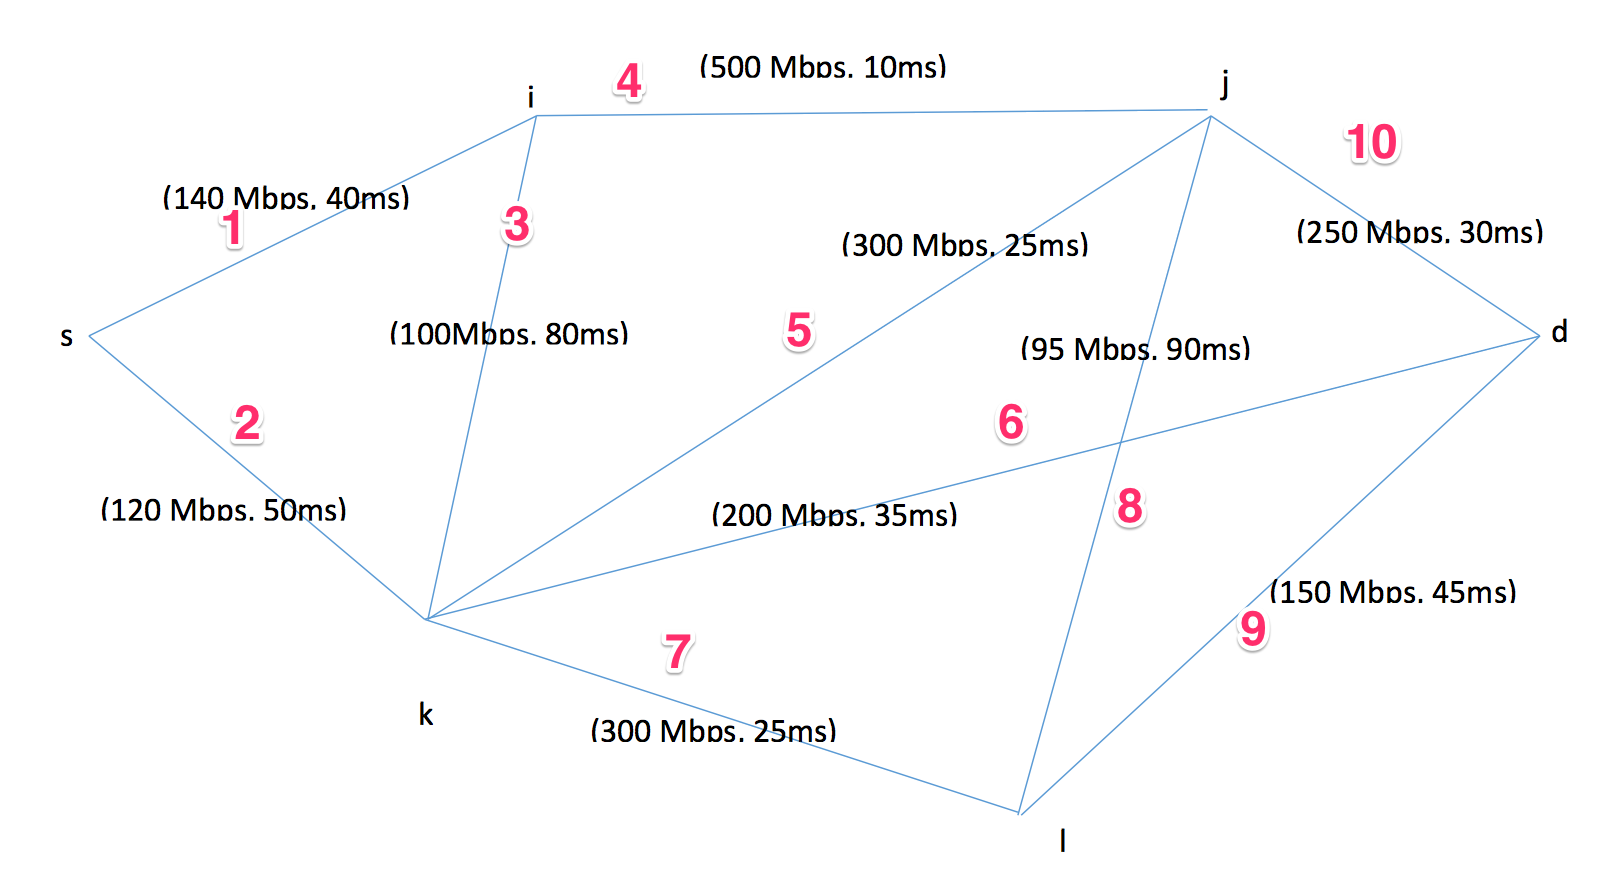
\includegraphics[width=0.8\textwidth]{labeled.png}
    \caption{Graph}
    \label{fig:graph}
\end{figure}

\textbf{Step 1: generate all paths from s to d that satisfy the bandwidth requirement.}

Noticed that there is only one link, Link 8, in the graph that has a bandwidth under 100 Mbs. Therefore, any paths including Link 8 will not satisfy the bandwidth requirement. When generating candidate paths, we exclude those paths which include Link 8. And all other generated paths satisfy the bandwidth requirement.

The paths generated are:
\begin{enumerate}
\item s-1-3-5-10-d
\item s-1-3-6-d
\item s-1-3-7-9-d
\item s-1-4-5-6-d
\item s-1-4-5-7-9-d
\item s-1-4-10-d
\item s-2-3-4-10-d
\item s-2-5-10-d
\item s-2-6-d
\item s-2-7-9-d
\end{enumerate}

\textbf{Step 2: keep paths that satisfy the latency requirement.}

What we do is, for each path listed above, sum up the total latency and exclude those with a total latency higher than 100 ms.

The remained paths are:
\begin{enumerate}
\item s-1-4-10-d
\item s-2-6-d
\end{enumerate}

In conclusion, the best paths that satisfy both requirements are:

\begin{enumerate}
\item s-(s,i)-(i,j)-(j,d)-d
\item s-(s,k)-(k,d)-d
\end{enumerate}


%%%%%%%%%%%%%%%%%%%%%%%%%%%%%%%%
\subsection{Hop-by-Hop routing Algorithm}

The link preference is to choose link with the highest bandwidth. The steps are listed as follows:

\begin{enumerate}
\item Start from origin s.
\item Choose Link 1 over Link 2.
\item Now we reaches node i. Choose Link 4 over Link 3.
\item Reaches node j. Choose Link 5 over Link 8 and Link 10.
\item Reaches node k. Choose Link 7 over Link 6.
\item Reaches node l. Choose Link 9 over Link 8.
\item Reaches destination d.
\end{enumerate}

However, the total latency of the above path 145ms which is greater than the restriction. This means that following this preference, the best path with all parameters at their optimal values does not exist.

Changing the link preference to choosing link with the lowest latency, this gives the same path as described above. And again, we reach the conclusion that the best path with all parameters at their optimal values does not exist.











